\section{Discussion}
\label{sec:discussion}

\subsection{No Quantum Advantage Under a Fair Comparison}
\label{sec:disc_advantage}

We set out to see how astronomical spectra could be classified with quantum machine
learning and to judge that honestly against the classical methods that already exist.
The starting point was sobering for any quantum ambition, since classical deep learning
already solves the coarse star-galaxy-quasar problem at around 99\% accuracy and
handles many subclasses well. We therefore moved relatively quickly to the harder fine-grained tasks,
beginning with the single hardest binary pair and then a four-class subset, and in each
case we built a quantum model and a classical counterpart of matched size and identical
surrounding pipeline.

The clearest lesson from both experiments is a simple one. When the classical baseline
is given the same care as the quantum model, it reaches the same accuracy. On the
binary pair the best quantum circuit and the best classical mirror are statistically
tied and on the four-class task the quantum head and a properly built classical head
of the same parameter count both reach about 96\%. We found no setting in either
experiment where a quantum model genuinely outperformed an equally well designed
classical one. The apparent exceptions all dissolved on inspection. The large early gap
on the binary task came from an under-built classical baseline and the collapse of the
small classical head on the four-class task was a dead-ReLU optimisation artefact that a
single change of activation removed. Once these were fixed the advantage disappeared.
If there is one practical takeaway, it is that the effort spent on the classical control
matters far more than the presence of a quantum circuit and that an apparent quantum
win should be treated as a hypothesis to be ruled out rather than a result.

\subsection{Parameter Efficiency and Class Balance}
\label{sec:disc_paramatch}

Going into the four-class task we hoped that a quantum head might at least prove more
parameter-efficient, reaching the same accuracy with fewer trainable weights even if it
offered no accuracy advantage. This did not hold up either. A small quantum head did
match a head with nine times as many parameters, but so did a classical head of the same
small size, which means the saving belongs to the strong frozen feature extractor that
feeds both rather than to the quantum circuit. The features it produces are already
separable enough that a tiny head of any kind suffices, so the parameter efficiency we
might have hoped to credit to the quantum circuit is really a property of the classical
front end.

What the quantum models did show, modestly, is a difference in class balance. Within the
family of circuits the wide and shallow shapes produced more balanced per-class recall
than the narrow and deep ones, halving the gap between the two classes on the binary
task. This is a real and slightly surprising effect, since wider circuits are usually
associated with harder training, but it is a difference in how the errors are
distributed rather than in overall accuracy, so we report it as an architectural
observation and not as a quantum advantage. The encoding analysis points the same way,
since the projection that chooses which few numbers reach the circuit matters far more
than the number of qubits, with a learned projection reaching 96\% while an unsupervised
one capped near 76\% on the very same circuit.
\subsection{Classical Limitations and Quantum Machine Learning Motivation}
The 62-class Baseline CNN shows a clear split between coarse and fine-grained
performance. The network separates the broad macro-categories well, as its
$92.51\%$ accuracy on the coarse 13-class GaSNet-II task indicates, but its
per-class recall drops substantially on fine-grained subclasses, falling as low as
$35.2\%$ for \texttt{STAR\_A5}. We report this as an observation about this
network on this dataset. It would take an architecture study we did not run to
establish that the limit is intrinsic to classical feature extractors rather than
specific to the model, the training budget or the label taxonomy we used.

Two patterns in the confusion matrix (Appendix~\ref{app:baseline_confusion}) are
consistent across runs. Symmetric confusion pairs such as \texttt{STAR\_A5}
$\leftrightarrow$ \texttt{STAR\_F0} and \texttt{QSO\_STARBURST} $\leftrightarrow$
\texttt{QSO\_STARBURST\_BROADLINE} suggest regions of the learned representation
where the two classes are not well separated in either direction, which is what
one would expect for classes that lie adjacent on a continuous physical sequence.
Separately, classes such as \texttt{STAR\_F0} and \texttt{GALAXY\_NORMAL} absorb
a large amount of foreign probability mass, behaving as sinks for spectra the
model cannot confidently assign. Whether a richer representation could resolve
these cases is precisely the open question, and it is what motivated us to target
these specific hard pairs in the Quantum Machine Learning experiments that
follow. We stress that this is a motivation for the experiments rather than a
prediction of their outcome.


\subsection{Spectral Attention of the Hybrid Model}
\label{sec:interpretability}

To check whether the hybrid model learns physically meaningful features rather than
arbitrary correlations, we apply two gradient-based interpretability methods to the
binary hybrid classifier. Grad-CAM on the last convolutional layer of the extractor
highlights the broad spectral regions the model relies on, and input saliency, the
gradient of the predicted class with respect to the raw flux, highlights the
individual wavelength bins. Both methods necessarily probe the classical CNN extractor
rather than the quantum circuit, since the circuit receives only the four compressed
features and has no notion of wavelength position. The analysis therefore shows where
in the spectrum the discriminative information is extracted, which is upstream of the
quantum stage. We run it on a broadline pair, \texttt{GALAXY\_AGN\_BROADLINE} against
\texttt{QSO\_STARBURST\_BROADLINE}, and average the heatmaps per class over the test
set, as shown in Figure~\ref{fig:gradcam}.

The Grad-CAM maps are localised and class-dependent. For the AGN class the attention
concentrates on a band that coincides with a strong broad emission peak in the mean
spectrum, while for the starburst quasar it shifts to the blue end of the continuum.
The input saliency by contrast is diffuse and stays high across most of the spectrum,
which reflects the known tendency of raw gradient saliency to be noisy and poorly
localised, so we read it only as a weak confirmation. Some Grad-CAM intensity also
sits at the extreme edges of the wavelength range, which is most likely a boundary
artefact of the convolution rather than a real feature.

\begin{figure*}[tbp]
    \centering
    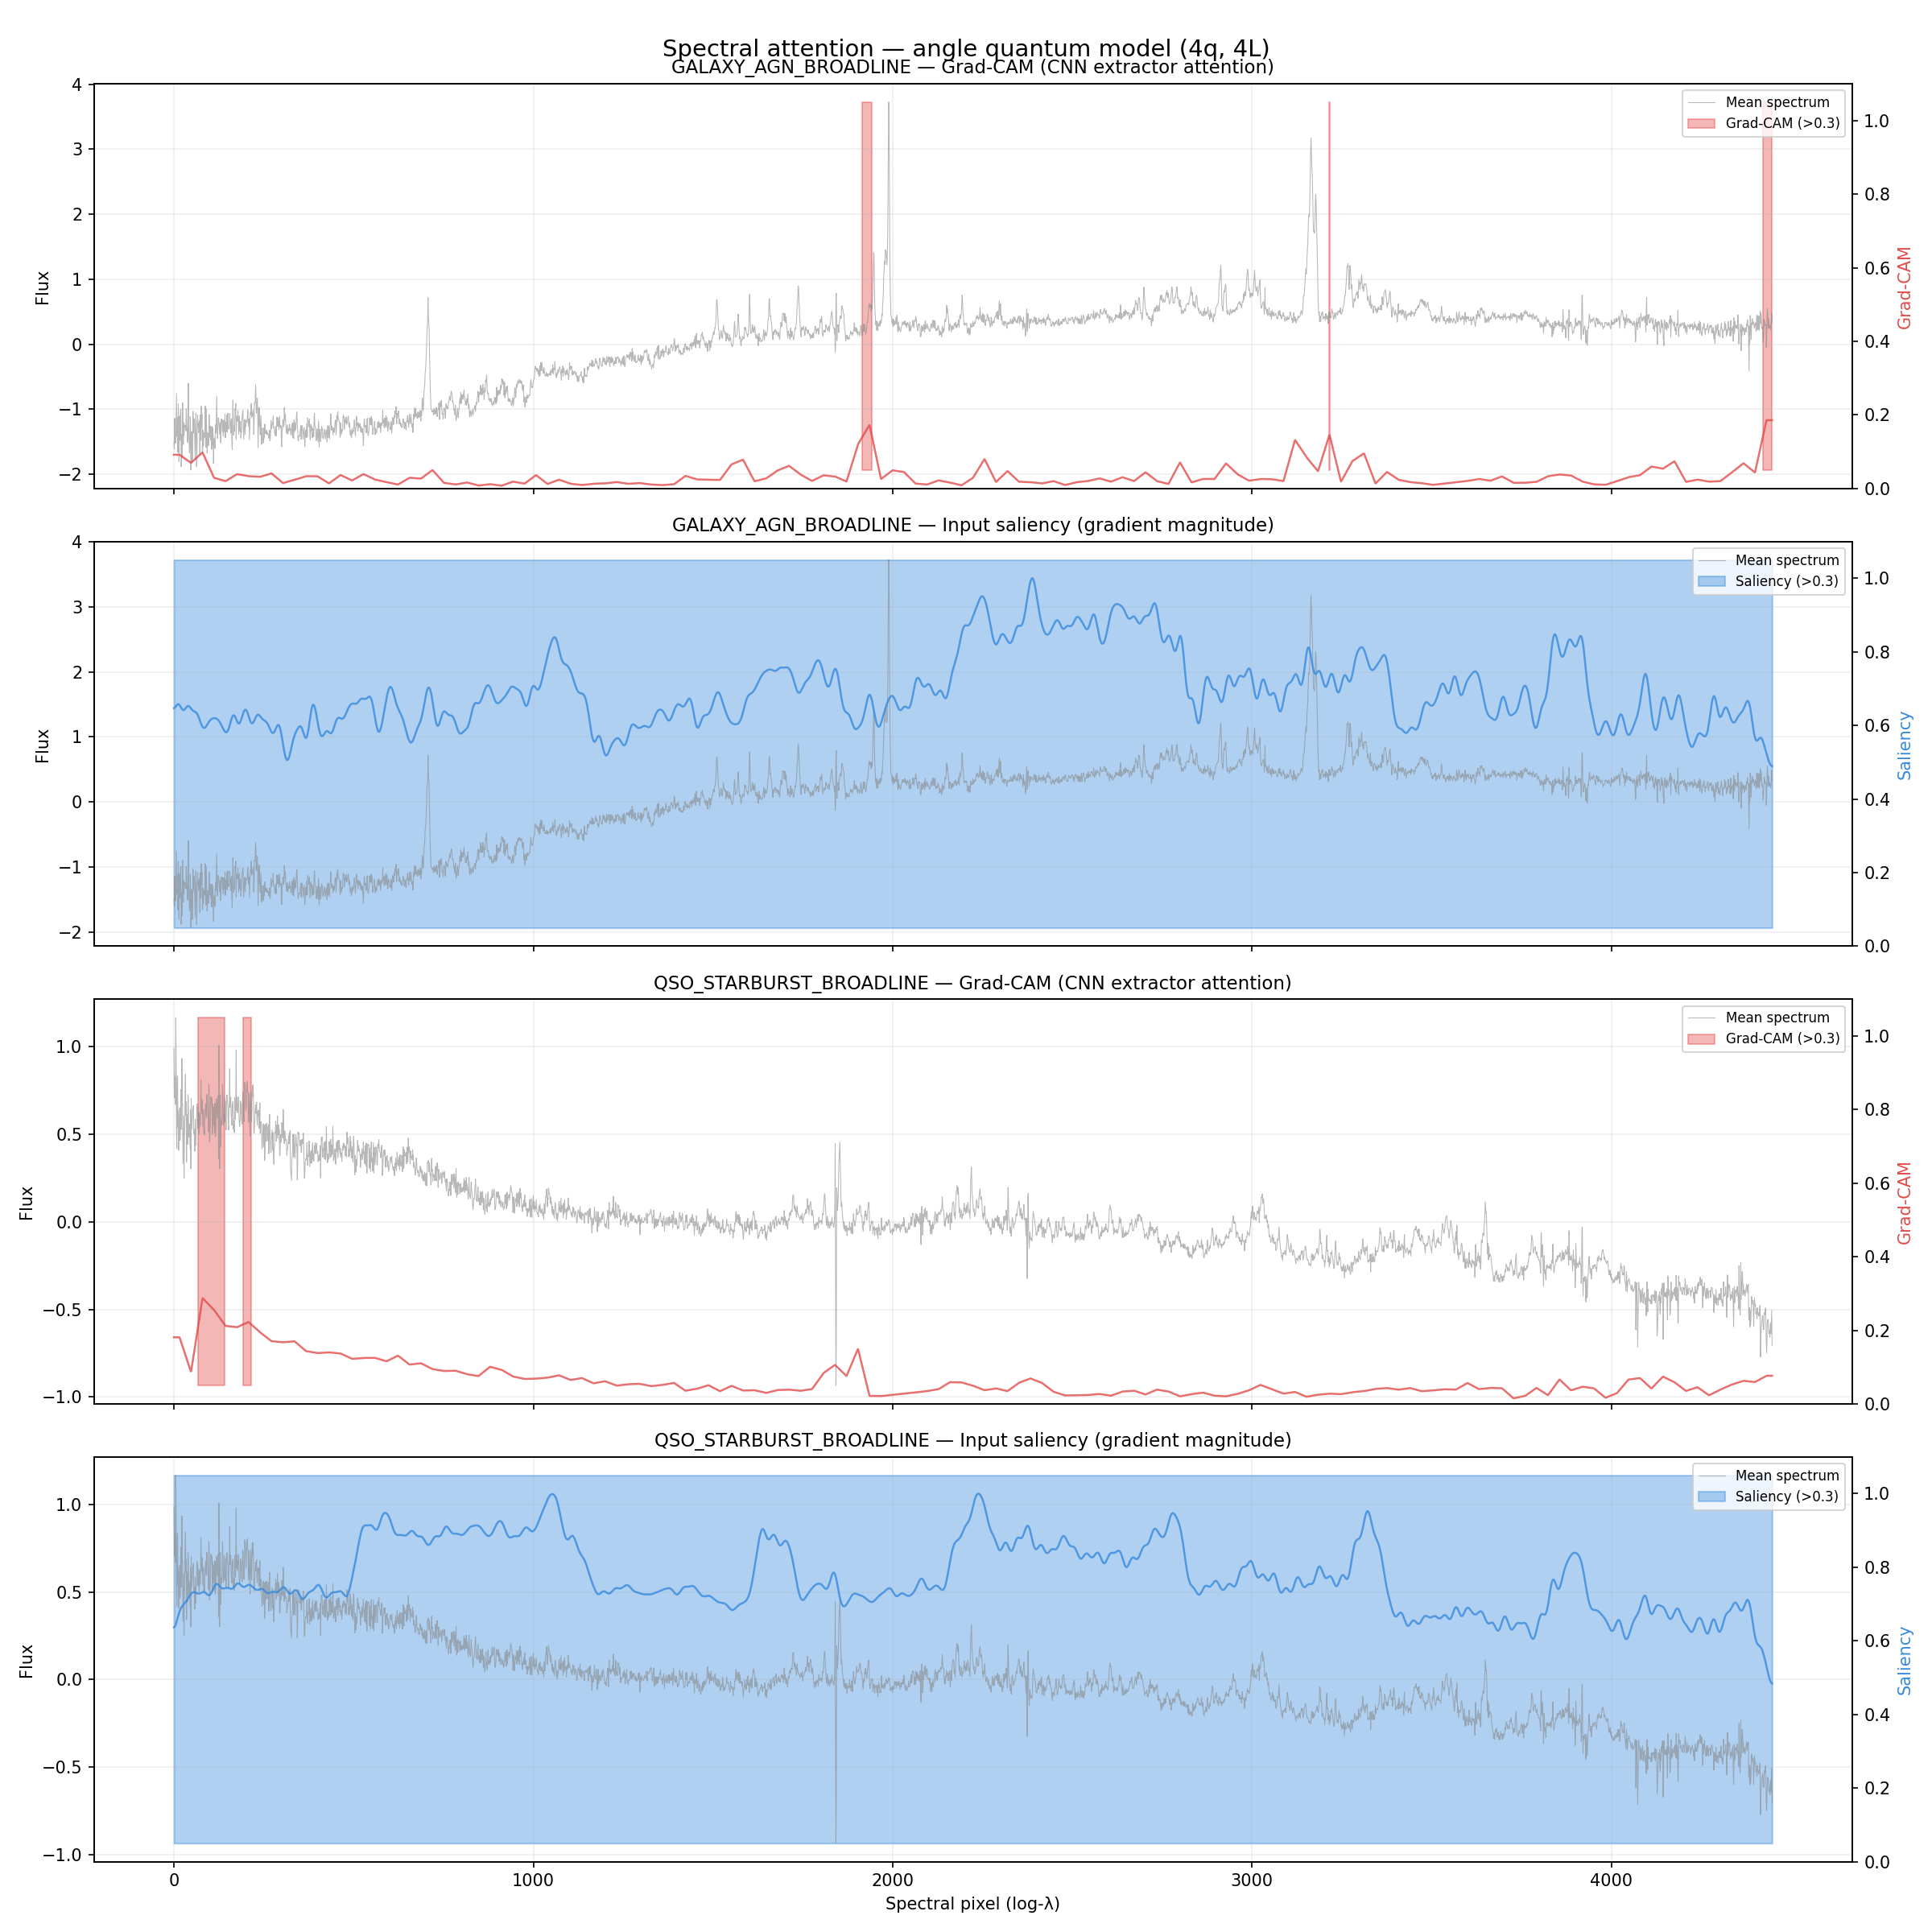
\includegraphics[width=0.92\textwidth]{Figures/gradcam_saliency_angle_4q.png}
    \caption{Per-class spectral attention of the binary hybrid model on
        \texttt{GALAXY\_AGN\_BROADLINE} against \texttt{QSO\_STARBURST\_BROADLINE}, averaged
        over the test set. For each class the upper panel shows Grad-CAM on the extractor's
        last convolutional layer and the lower panel shows input-gradient saliency, both
        overlaid on the mean spectrum. Grad-CAM localises to a broad emission band for the AGN
        class and to the blue continuum for the quasar, whereas the raw saliency is diffuse.
        Both methods probe the classical extractor, since the quantum circuit receives only
        four scalar features.}
    \label{fig:gradcam}
\end{figure*}

What makes this result reassuring is that the regions the model relies on are the
ones that established spectral classification also keys on. These two classes are
separated physically by their broad emission lines and by the slope of their continuum. Broadline objects are
defined by exactly these wide emission features, and a blue quasar continuum looks
clearly different from the redder galaxy continuum. The long-standing template-fitting
pipelines that classify SDSS spectra key on the same structure, matching an observed
spectrum against templates whose emission lines and continuum shape encode the
class~\cite{bolton2012boss}. That the model concentrates on these features, and not
on flat or noise-dominated regions, is therefore reasonable evidence that it has
picked up genuinely discriminative structure rather than a spurious shortcut,
although attribution methods show where a model looks and not why, so we do not
treat this as proof that no shortcut is present.

That the model concentrates on emission lines and the continuum slope is not only
physically intuitive but is what an optimal classifier should do. To make this precise
we model a preprocessed spectrum as a vector $x \in \mathbb{R}^{L}$ over its $L$
wavelength bins and assume that the two classes have Gaussian class-conditional
distributions with class means $\mu_0, \mu_1 \in \mathbb{R}^{L}$ and a shared
covariance $\Sigma$,
\begin{equation}
    x \mid y = c \;\sim\; \mathcal{N}(\mu_c, \Sigma), \qquad c \in \{0, 1\}.
    \label{eq:gauss}
\end{equation}
Under this model the Bayes-optimal decision rule is linear and is given by Fisher's
linear discriminant, which assigns $x$ to class~1 when $w^{\ast\top} x + b > 0$ with
\begin{equation}
    w^{\ast} = \Sigma^{-1}(\mu_1 - \mu_0).
    \label{eq:fisher}
\end{equation}
The vector $w^{\ast}$ is also the weight that any well-trained differentiable
classifier approximates, since for a model $f(x)$ that estimates the log-odds
$\log\!\big(p(y=1\mid x)/p(y=0\mid x)\big)$ the input saliency is exactly
$\nabla_x f(x) = w^{\ast}$ in this linear regime. The saliency the network learns is
therefore the discriminant direction itself.

To read off the importance of a single wavelength bin we neglect cross-bin
correlations and approximate the covariance as diagonal,
$\Sigma \approx \operatorname{diag}(\sigma_1^2, \dots, \sigma_L^2)$. The per-bin weight
then reduces to
\begin{equation}
    w^{\ast}_i = \frac{\mu_{1,i} - \mu_{0,i}}{\sigma_i^2},
    \label{eq:weight}
\end{equation}
and the contribution of bin $i$ to the squared Mahalanobis separation between the
classes is the per-bin Fisher ratio, the squared signal-to-noise of that bin,
\begin{equation}
    J_i = \frac{(\mu_{1,i} - \mu_{0,i})^2}{\sigma_i^2},
    \qquad
    (\mu_1 - \mu_0)^{\top}\Sigma^{-1}(\mu_1 - \mu_0) = \sum_{i=1}^{L} J_i .
    \label{eq:fisherratio}
\end{equation}
The sum in \eqref{eq:fisherratio} is the total class separability, and each $J_i$ is
the additive share contributed by bin $i$. It is maximised precisely at the wavelength
bins where the two class-mean spectra differ most relative to their variance. For the
broadline pair studied here those bins are the broad emission lines, where one class
carries a strong line that the other lacks, and the continuum slope, which separates
the blue quasar from the redder galaxy. The Bayes-optimal classifier therefore places
almost all of its weight on exactly the regions that Grad-CAM and the saliency analysis
highlight in Figure~\ref{fig:gradcam}. The agreement between the learned attention and
the optimal discriminant $w^{\ast}$ is the sense in which looking at these spectral
regions is not an arbitrary choice but the mathematically correct way to separate the
two classes.

This also reinforces the structural reading of our hybrid models, but it needs to be
stated carefully. The hard part of the task is feature extraction, deciding which
parts of the spectrum matter, and only the classical front end can do this, since the
quantum circuit never receives the wavelength axis and sees just a handful of
already-compressed numbers. The discriminant $w^{\ast}$ of \eqref{eq:fisher} makes
the same point formally: it is a function of the raw spectrum, so the classical
extractor is the only component of our pipeline that could represent it. The head that follows, quantum or classical, still has a
job to do, namely mapping those features to a decision, and it has to be built
competently. The collapse of the dead-ReLU control in the four-class
experiment makes this clear, since a poorly built head fails even on good features. What that same experiment also
shows is that the head can be small and that its quantum-versus-classical nature makes
no difference once the features are good, since a 556-parameter head matched a
nine-times-larger one as soon as it used a robust activation. The picture is therefore
not that the head is irrelevant, but that the discriminative work of finding the right
spectral features happens in the classical extractor, while the head only has to use
them, which is consistent with the parity between the quantum and classical heads found
in both experiments.

\subsection{Limitations}
\label{sec:limitations}

Several limitations bound these conclusions. All quantum models were run on a noiseless
classical statevector simulator rather than on real hardware. For the variational and
kernel methods studied here this is the most favourable setting, since real devices add
noise, shot statistics and decoherence that can only degrade a circuit trained to
implement a specific unitary, so the absence of an advantage here is if anything a
stronger result than it would be on hardware. We note that this reasoning is specific to
the model families we test and does not generalise to all of quantum machine learning;
in quantum reservoir computing, for instance, device noise and dissipation form part of
the computational resource rather than a nuisance, so a noiseless simulator would not be
the most favourable setting there. The
circuits were also restricted to eight qubits or fewer, which is realistic for
near-term devices but limits how much of each spectrum the quantum stage can ever see.
The study covers a single scientific domain, the SDSS spectra, and a small number of
hard class pairs rather than the full survey. Finally, the quantum circuit is a tiny
fraction of each model, a few dozen parameters against tens of thousands in the
classical stages, so the experiments test one specific hybrid regime rather than
quantum machine learning in general and the seed counts in the sweep are modest, so
the small differences between configurations should be read as indicative rather than
conclusive.


\subsection{Absence of Quantum Advantage in Few-Shot SVM Classification}
The results of \hyperref[sec:exp3_results]{Experiment 3} demonstrate the absence of a
practical quantum advantage for a QSVM operating directly on pooled raw flux. The finding
is more nuanced than a simple classical win. Reported at the encoding bandwidth most
favourable to it, the fidelity kernel is marginally ahead of the tuned classical RBF
baseline on the point estimate for every training-set size up to $n = 50$, but the
confidence intervals overlap throughout and the pre-registered criterion is never met, so
the honest reading of the few-shot regime is parity. The ordering then reverses: as the
training set grows the classical kernel pulls significantly ahead, and the projected
kernel trails both. What the experiment rules out is therefore not a small quantum edge in
the data-starved corner, but a quantum advantage that survives scrutiny and scales.

This outcome can be analyzed through the theoretical constraints of the respective kernel spaces. The classical RBF kernel implicitly maps input vectors into an infinite-dimensional functional space. This continuous, unconstrained mapping is highly effective at establishing linear decision boundaries within complex, highly correlated data manifolds, such as the pooled spectral bins used here.

In contrast, the QSVM feature map is strictly bounded by the dimensionality of its corresponding Hilbert space. For the optimal feature set of $f=12$, the quantum circuit explores a $2^{12}$-dimensional space. While theoretically vast, the expressivity of this space is governed by discrete parameterized rotations and Pauli expansions, and it is fixed once the feature map is chosen. This is a plausible explanation for the specific shape of the result, namely that the quantum kernels keep pace while data is scarce and fall behind once it is not: the rigid, periodic quantum feature map cannot refine itself as more samples arrive, whereas the tuned RBF kernel continues to exploit the geometric flexibility of its infinite-dimensional space. We offer this as an interpretation consistent with our measurements rather than as a demonstrated mechanism, since we did not vary the feature map systematically enough to isolate it. What the data does show plainly is that the quantum feature map separated the symmetric confusion pairs (for example the starburst and star-forming subclasses) no better than the classical kernel.

The geometric-difference pre-screen is instructive here, though not in the way we initially
expected. At the reported bandwidth neither kernel is geometrically degenerate
($g(K_C \| K_Q) = 3.95$ for the fidelity kernel and $17.68$ for the projected kernel), so
the diagnostic of Huang et al. \cite{huang2021power} does not predict the null result in
advance: on this measure both quantum kernels induce a similarity structure that a
classical RBF kernel does not trivially reproduce. That distinctness simply fails to pay
off. The clearest illustration is that the projected kernel, by far the more geometrically
distinct of the two, is also the weaker classifier at nearly every sample size. A large
geometric difference is thus a necessary but far from sufficient condition for a practical
separation, and we regard this as the more useful methodological lesson than the screen's
intended role as an early stopping criterion. The metric is also strongly
encoding-dependent, dropping to $g = 1.89$ for the same kernel at a different bandwidth,
which means it characterises the chosen feature map at least as much as it characterises
the data.

\subsection{Interpreting the Absence of a Quantum Advantage}
\label{sec:discussion_exp4}

Experiment~4 found no robustness advantage for the Quanvolutional filter over a classical baseline under strict parameter parity. Three observations constrain this null result.

First, training the variational circuit provided no benefit. Under the heavy head, a frozen random circuit performed as well as the trained version; only after removing the deep head did training show any effect. This suggests that a deep classical aggregator renders the quantum layer an effectively fixed nonlinear embedding—the specific circuit parameters matter little for final accuracy.

Second, the light-head ablation reveals where the filters differ. Removing the deep head degraded both models, but the quantum filter degraded more, showed higher variance across seeds, and was significantly worse under adversarial training ($p=0.014$). The quantum feature map is thus less linearly separable and less stable in a shallow regime than the classical filter.

Third, the Jacobian analysis does not support an intrinsic-smoothness interpretation. As reported in Section~\ref{sec:exp4_results} and Figure~\ref{fig:exp4_jacobian_dists}, the ordering of smoothness reverses between the two configurations: under the heavy head the quantum filter is significantly smoother ($0.747$ versus $1.052$ for OOD, $p=0.006$), while under the light head the classical filter has the lower median norm ($0.282$ versus $0.559$). Because the probe acts on trained weights, it characterises the learned solution in each regime rather than a fixed property of the circuit.

In summary, for 1D spectral classification under a fair parameter budget, this hybrid design yields no robustness advantage over a matched classical filter. The high accuracy of the heavy-head network is attributable to its classical components.

% ==========================================
% DISCUSSION SECTION (Experiment 5 additions)
% ==========================================
\subsection{True QCNNs on Classical Data: Inductive Bias under a Budget}
\label{sec:discussion_exp5}

Experiment~5 serves as a negative control. The QCNN architecture \cite{cong2019qcnn} was designed to exploit structures native to quantum states, guaranteeing the absence of barren plateaus \cite{pesah2021absence}. Embedding classical astronomical flux removes this foundational premise. Consequently, we observe no absolute quantum advantage over an unconstrained classical network.

However, the experiment reinforces the necessity of parameter-matched baselines.
The comparison involves two classical controls, introduced in
Section~\ref{sec:exp5_results}: the \emph{Tiny CNN} is a severely constrained 1D
convolutional network of roughly $100$ trainable weights, chosen to match the
QCNN's budget exactly and therefore serving as the strict-parity control, while
the \emph{Huge CNN} is an unconstrained $8228$-parameter network that marks the
upper bound of classical performance on the same data.

Against these two the picture depends on which metric is read, and it is worth
separating them. On clean accuracy the QCNN is ahead of the Tiny CNN in all four
quadrants, and the margin is large where data is scarce ($0.52$ versus $0.31$ in
Q3 and $0.48$ versus $0.29$ in Q4, against a chance level of $0.25$). On
robustness AUC the ordering is less uniform: the QCNN leads in Q2, Q3 and Q4 but
\emph{trails} the Tiny CNN in Q1 ($0.408$ versus $0.462$), and of the four
comparisons only Q4 reaches significance ($p = 0.027$; see
Table~\ref{tab:exp5_wilcoxon}). The Hybrid QCNN is the more consistent of the two
quantum models against strict parity. We would therefore not claim that the QCNN
dominates its matched control outright; the defensible statement is that under a
tight parameter budget the quantum models remain usable in regimes where the
matched classical network collapses, while the unconstrained Huge CNN remains
ahead on clean accuracy throughout. This points to the data-starved, heavily
constrained regime as the place where a quantum inductive bias might matter,
though four quadrants on one dataset can only be suggestive.

This few-shot behaviour is at least consistent with the direction of the bound of
Caro et al.~\cite{caro2022generalization}, who show that the generalization error
of a variational model scales with the number of trainable gates. The quantum
core in question is the weight-shared hierarchy described in
Section~\ref{sec:exp5_arch}, alternating $SU(4)$ convolution blocks with coherent
pooling as the register is reduced from twelve qubits to six and then to three,
followed by a linear readout, for roughly $101$ trainable parameters in total.
That core retains usable accuracy at twenty samples per class, whereas the
similarly sized classical filter overfits and collapses towards chance. We note
that the bound is stated in trainable gates rather than parameters and was
derived for a different setting, so we read the agreement as qualitative support
rather than as a quantitative confirmation. On our evidence the QCNN's inductive
bias shows up as sample efficiency under a strict capacity budget rather than as
scalable representational power.

The encoding ablation points to state preparation as the source of the pure
QCNN's fragility. Because both variants share the same convolution and pooling
blocks and differ only in how the spectrum is loaded, the hybrid model's higher
robustness AUC in all four quadrants is most readily explained by the encoding
rather than by the quantum architecture. A mechanism is available: distributing
the raw 4096-bin spectrum across a globally $L_2$-normalised state lets
high-frequency noise reshape the entire amplitude vector at once
\cite{schuld2021encoding}, whereas classically-assisted angle encoding confines
the perturbation to bounded, localised rotations. With a single ablation on one
dataset we regard this as strong evidence for the encoding being the weak point
in our setup, though not as a general statement about amplitude encoding.

Finally, the Jacobian analysis is consistent with textbook capacity dynamics
\cite{szegedy2013intriguing, sokolic2017robust}. The measurements are collected
in Table~\ref{tab:exp5_jacobian} and Figure~\ref{fig:exp5_jacobian}. Under clean
high-data training (Q1) the over-parameterised Huge CNN has by far the roughest
map, with a median spectral norm of $5.73$ against $3.52$ for the QCNN, and it is
also the least robust model in that quadrant, so smoothness and robustness move
together there. The effect is regime-dependent rather than a fixed property of
the architecture. Adversarial training flattens every model's Jacobian, with all
four dropping to between $1.90$ and $2.36$ in Q2, which compresses the
differences between them. In the few-shot quadrants the Tiny CNN reaches the
smallest norm of any model ($0.19$ in Q3 and $0.18$ in Q4), but this cannot be
read as robustness, since the same model sits near chance accuracy there; the
near-zero norm reflects collapse to an almost constant function. Smoothness is
therefore only interpretable alongside accuracy, and we would not treat a low
Jacobian norm on its own as evidence of a well-behaved model.

Ultimately, this experiment concludes the QML sequence with a consistent structural finding: across feature extraction, kernel methods, and fully coherent convolutions, variational quantum models achieve classical parity under matched conditions. Their distinct characteristics emerge in sample efficiency, regularization, and encoding sensitivity, rather than raw top-line dominance over unconstrained classical architectures.
